%----------------------------------------------------------
\def\notedate{2021.12.04}
\def\currentauthor{Ершов В. (РК6-72Б)}
%----------------------------------------------------------
\notestatement{rndhpcedt}{Краткое описание алгоритма визуализации графа}

В ходе разработки web-ориентированного редактора графов, который позволяет импортировать и экспортировать файлы в формате aDOT~\cite{SokADOT}, был разработан алгоритм визуализации графов. В этой заметке будет рассмотрен этот алгоритм и приведено несколько примеров aDOT файлов, которые корректно визуализируются, используя этот алгоритм.

Теоретические основы и назначение графоориентированной программной инженерии представлены в работе~\cite{SokPersh2018GBSE}. Принципы применения графоориентированного подхода зафиксированы в патенте~\cite{patentRU2681408}. 

Один из самых важных критериев построенного графа -- это его читаемость. Граф должен быть построен корректно и недопускать неоднозначностей при его чтении. Например, вершины не должны налегать друг на друга, ребра не должны пересекаться, создавая сложные для восприятия связи.

Проведя длительную аналитическую работу, было принято решение разбивать граф по уровням. Рассмотрим следующее aDOT-определение графовой модели \textsf{G} (листинг~\ref{lst:gm.exmpl.1}).

\begin{lstlisting}[frame=single, label={lst:gm.exmpl.1}, caption={Пример aDOT-определение простейшей графовой модели \textsf{G}}, language=aDOTExample]
digraph G {
// Parallelism
	s1 [parallelism=threading]
// Graph definition
	__BEGIN__ -> s1
	s4 -> s6 [morphism=edge_1]
	s5 -> s6 [morphism=edge_1]
	s1 => s2 [morphism=edge_1]
	s1 => s3 [morphism=edge_1]
	s2 -> s4 [morphism=edge_1]
	s3 -> s5 [morphism=edge_1]
	s6 -> __END__ 
}
\end{lstlisting}

Если нарисовать такой граф на бумаге, то становится очевидно, что каждый набор вершин имеет одну координату по оси X, а связанные с ними вершины находятся правее по координате X, таким образом напрашивается разбиение графа по уровням. На рисунке (\ref{fig:graph_levels}) представлен этот граф, разбитый на уровни.

\begin{figure}[ht!]
\center{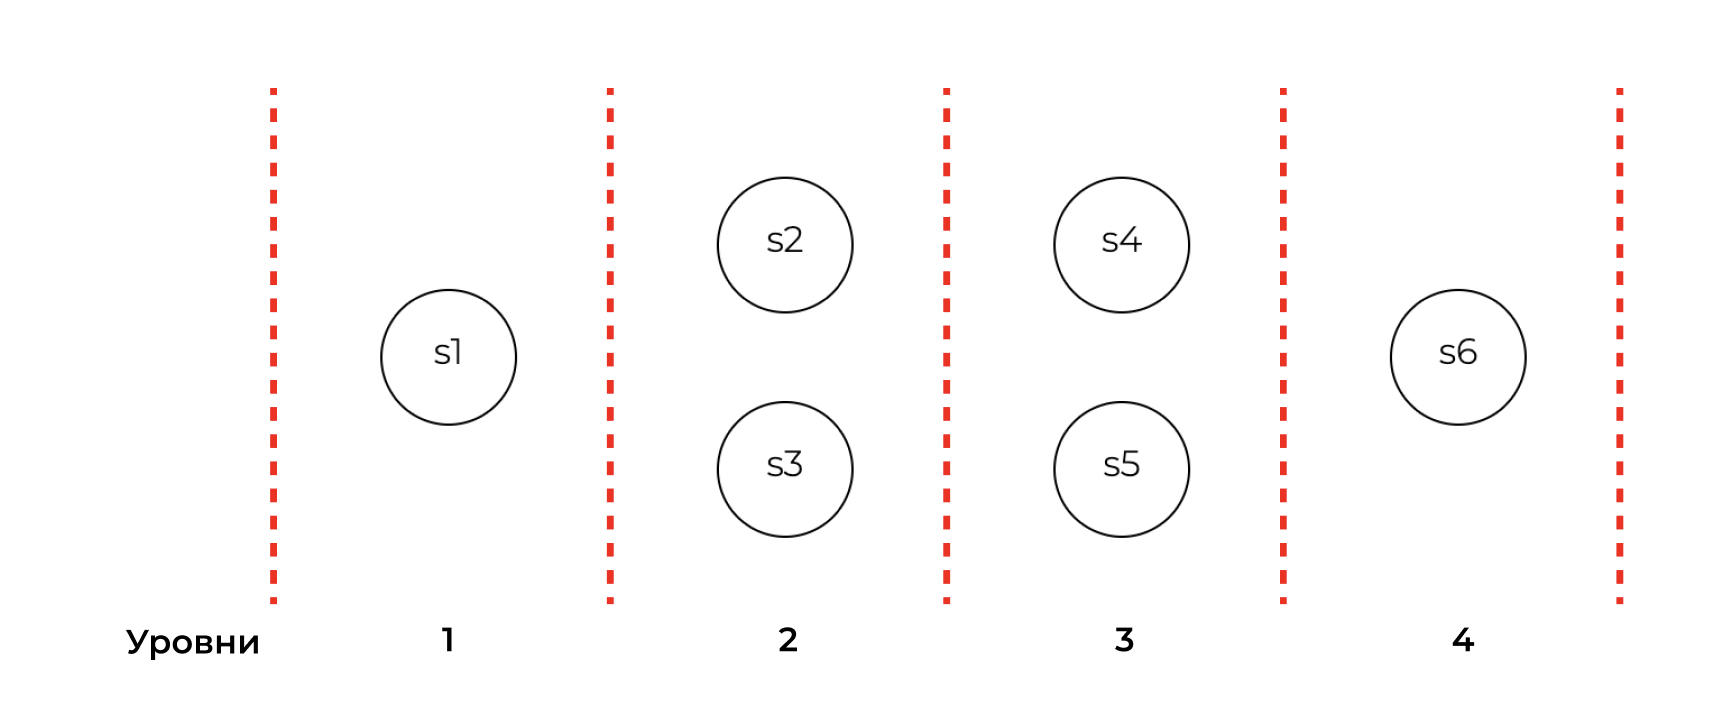
\includegraphics[width=0.8\linewidth]{ResearchNotes/rndhpc_not_edt_2021_12_04/graph_levels.png}}
\caption{Узлы графовой модели \textsf{G}, представленные на разных ``уровнях''}
\label{fig:graph_levels}
\end{figure}

Разбиение графа по уровням является основой алгоритма визуализации, далее на примере более сложного графа поэтапно разберем алгоритм.

Рассмотрим следующий файл на языке aDOT (листинг~\ref{lst:gm.exmpl.2}).

\begin{lstlisting}[frame=single, label={lst:gm.exmpl.2}, caption={Пример aDOT-определения графовой модели \textsf{TEST}}, language=aDOTExample]
digraph TEST
{
// Parallelism
	s11 [parallelism=threading]
	s4 [parallelism=threading]
	s12 [parallelism=threading]
	s15 [parallelism=threading]
	s2 [parallelism=threading]
	s8 [parallelism=threading]
// Functions
	f1 [module=DEFAULT_VALUE, entry_func=DEFAULT_VALUE]
// Predicates
	p1 [module=DEFAULT_VALUE, entry_func=DEFAULT_VALUE]
// Edges
	edge_1 [predicate=p1, function=f1]
// Graph model description
	__BEGIN__ -> s1
	s6 -> s8 [morphism=edge_1]
	s7 -> s8 [morphism=edge_1]
	s10 -> s8 [morphism=edge_1]
	s11 => s8 [morphism=edge_1]
	s11 => s9 [morphism=edge_1]
	s14 -> s9 [morphism=edge_1]
	s3 -> s9 [morphism=edge_1]
	s4 => s6 [morphism=edge_1]
	s4 => s7 [morphism=edge_1]
	s4 => s10 [morphism=edge_1]
	s4 => s11 [morphism=edge_1]
	s12 => s4 [morphism=edge_1]
	s12 => s14 [morphism=edge_1]
	s13 -> s3 [morphism=edge_1]
	s15 => s14 [morphism=edge_1]
	s15 => s14 [morphism=edge_1]
	s2 => s12 [morphism=edge_1]
	s2 => s13 [morphism=edge_1]
	s2 => s15 [morphism=edge_1]
	s1 -> s2 [morphism=edge_1]
	s8 => s9 [morphism=edge_1]
	s8 => s6 [morphism=edge_1]
	s9 -> __END__ 
}
\end{lstlisting}

В результате визуализации модели будет получен граф, представленный на рисунке (\ref{fig:main_graph}).

\begin{figure}[ht!]
\center{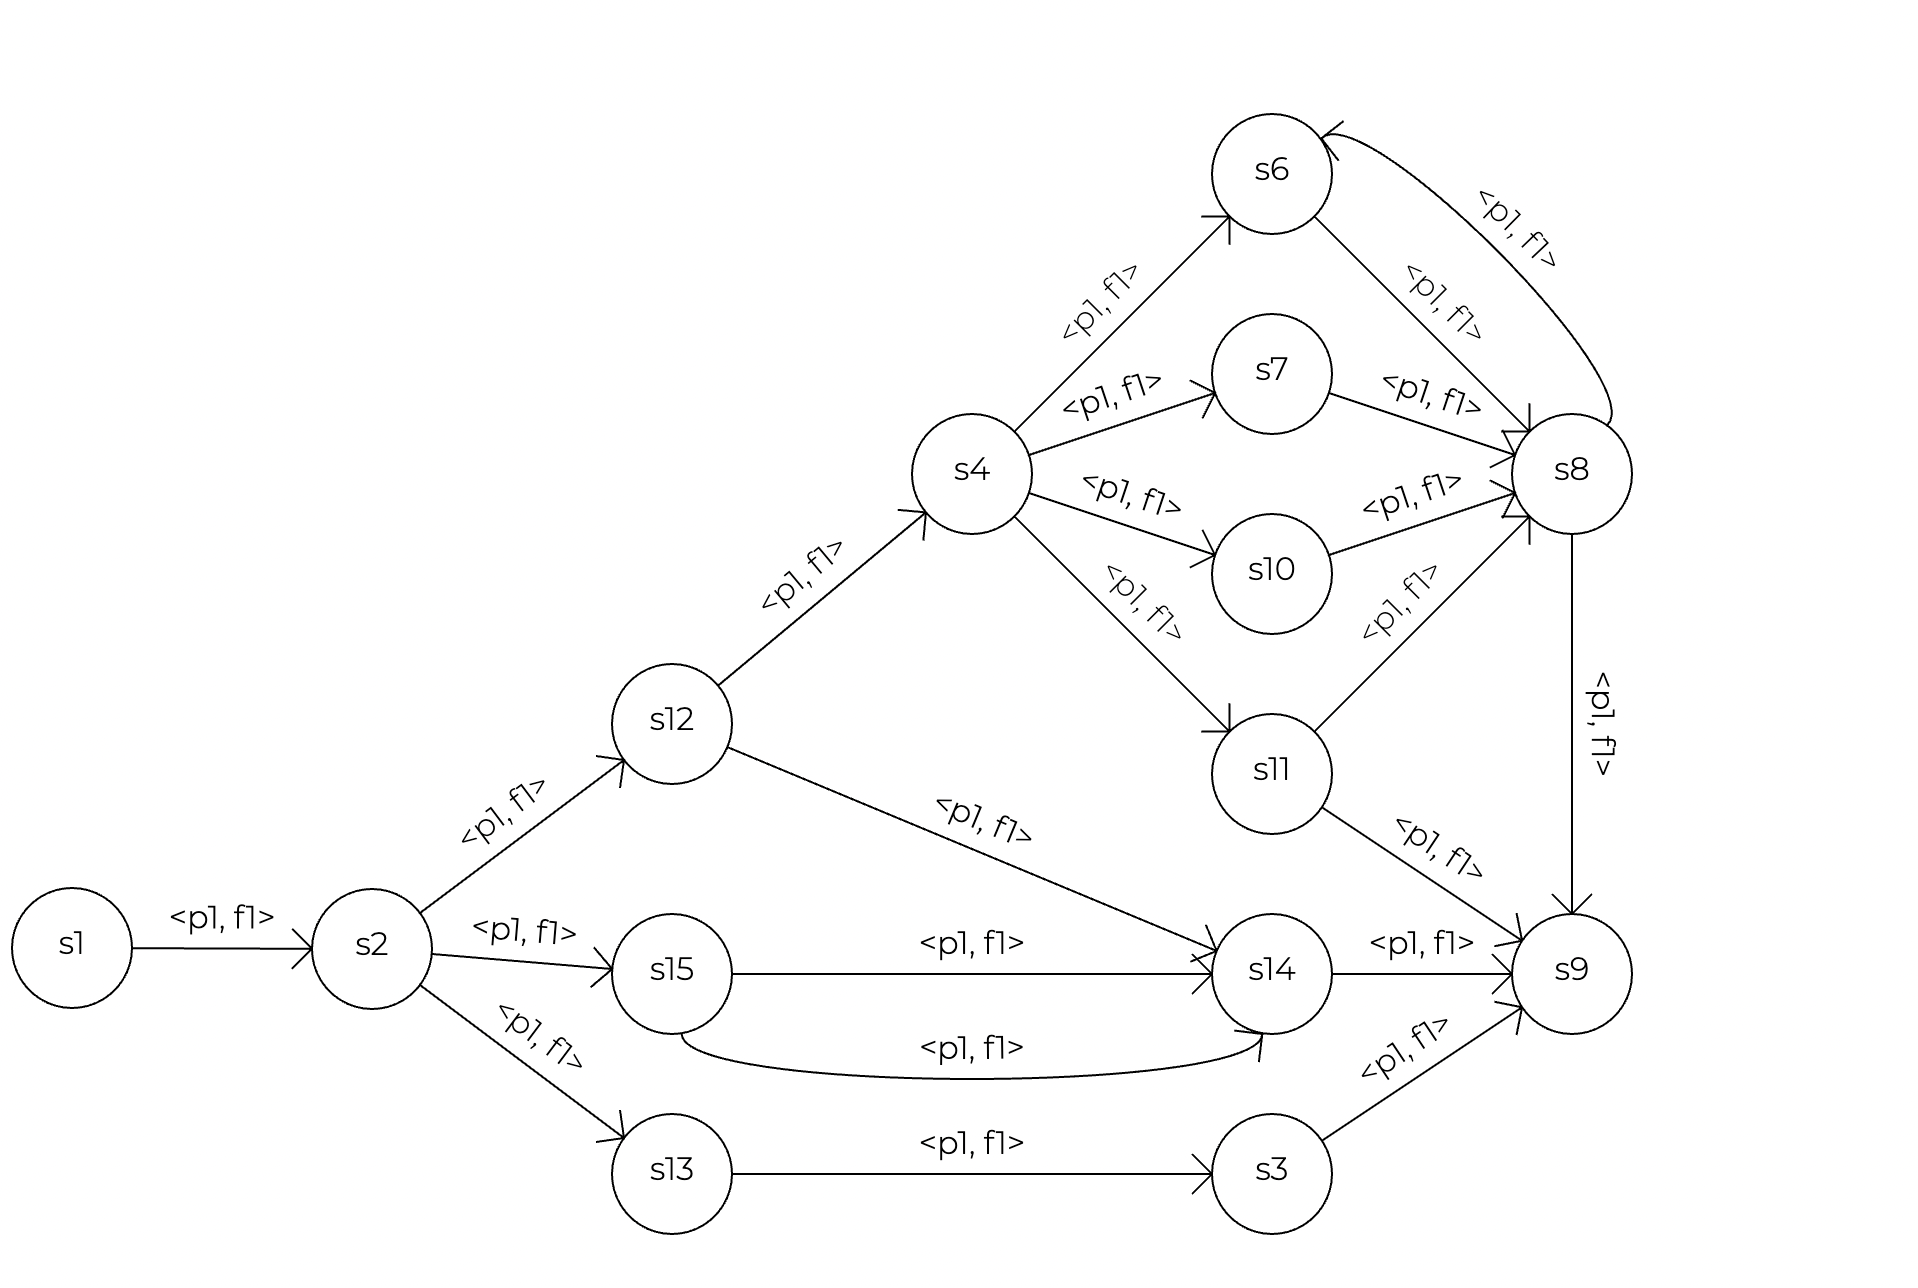
\includegraphics[width=0.85\linewidth]{ResearchNotes/rndhpc_not_edt_2021_12_04/main_graph.png}}
\caption{Визуализация графовой модели \textsf{TEST}}\label{fig:main_graph}
\end{figure}

Основная задача алгоритма -- это отрисовать вершины графа в корректных позициях, а затем построить между ними ребра. Поскольку редактор графов -- это web-ориентированное приложение, то вся бизнес-логика написана на языке \textsf{JavaScript}. В \textsf{JavaScript} имеется очень удобный инструмент -- объекты. Аналогами объектов в других языках программирования являются хэш-карты, но в Javascript возможности использования объектов гораздо шире. Всю информацию об уровнях графа будем хранить в объекте levels. Ниже представлено как выглядит объект levels для рассматриваемого выше графа:

\begin{verbatim}
{
	"1":[{"s1":[]}],
	"2":[{"s2":["s1"]}],
	"3":[{"s12":["s2"]}, {"s13":["s2"]}, {"s15":["s2"]}],
	"4":[{"s4":["s12"]}],
	"5":[{"s9":["s14","s3"]}, {"s6":["s4"]}, {"s7":["s4"]}, {"s10":["s4"]}, 
	{"s11":["s4"]},	{"s14":["s12","s15"]}, {"s3":["s13"]}],
	"6":[{"s8":["s6","s7","s10","s11"]}, {"s9":["s11","s14","s3"]}]
}
\end{verbatim}

Ключами объекта levels являются номера уровней, представленные в формате string. Свойсвами являются массивы, на один уровень - один массив. Каждый элемент массива содержит информацию об одной вершине на этом уровне, следовательно количество вершин на уровне - это размер массива. Далее заметим, что элемент массива это не просто string с названием вершины, а объект. Этот объект содержит один ключ - название вершины на этом уровне, а свойством является массив, который содержит список вершин из которых перешли в эту вершину (переход только по одному ребру).

В качестве примера рассмотрим уровень 5 объекта levels, который был представлен ранее.

\begin{minipage}{0.5\textwidth}
	\begin{verbatim}
	{
	  "5":[{"s9":["s14","s3"]}, {"s6":["s4"]}, {"s7":["s4"]}, 
	  {"s10":["s4"]}, {"s11":["s4"]}, {"s14":["s12","s15"]}, {"s3":["s13"]}],
	}
	\end{verbatim}
\end{minipage}


Уровень 5 в графе представлен 7-ю вершин: ``s9'', ``s6'', ``s7'', ``s10'', ``s11'', ``s14'', ``s3''. Например, в вершину ``s6'' мы пришли из вершины ``s4'', таким образом, по ключу ``s6'' находится массив c один элементом ``s4''
\begin{verbatim}
{"s6": ["s4"]}
\end{verbatim}

На рисунке (\ref{fig:main_graph_level5}) представлен граф с выделенным уровнем №5.

\begin{figure}[ht!]
\center{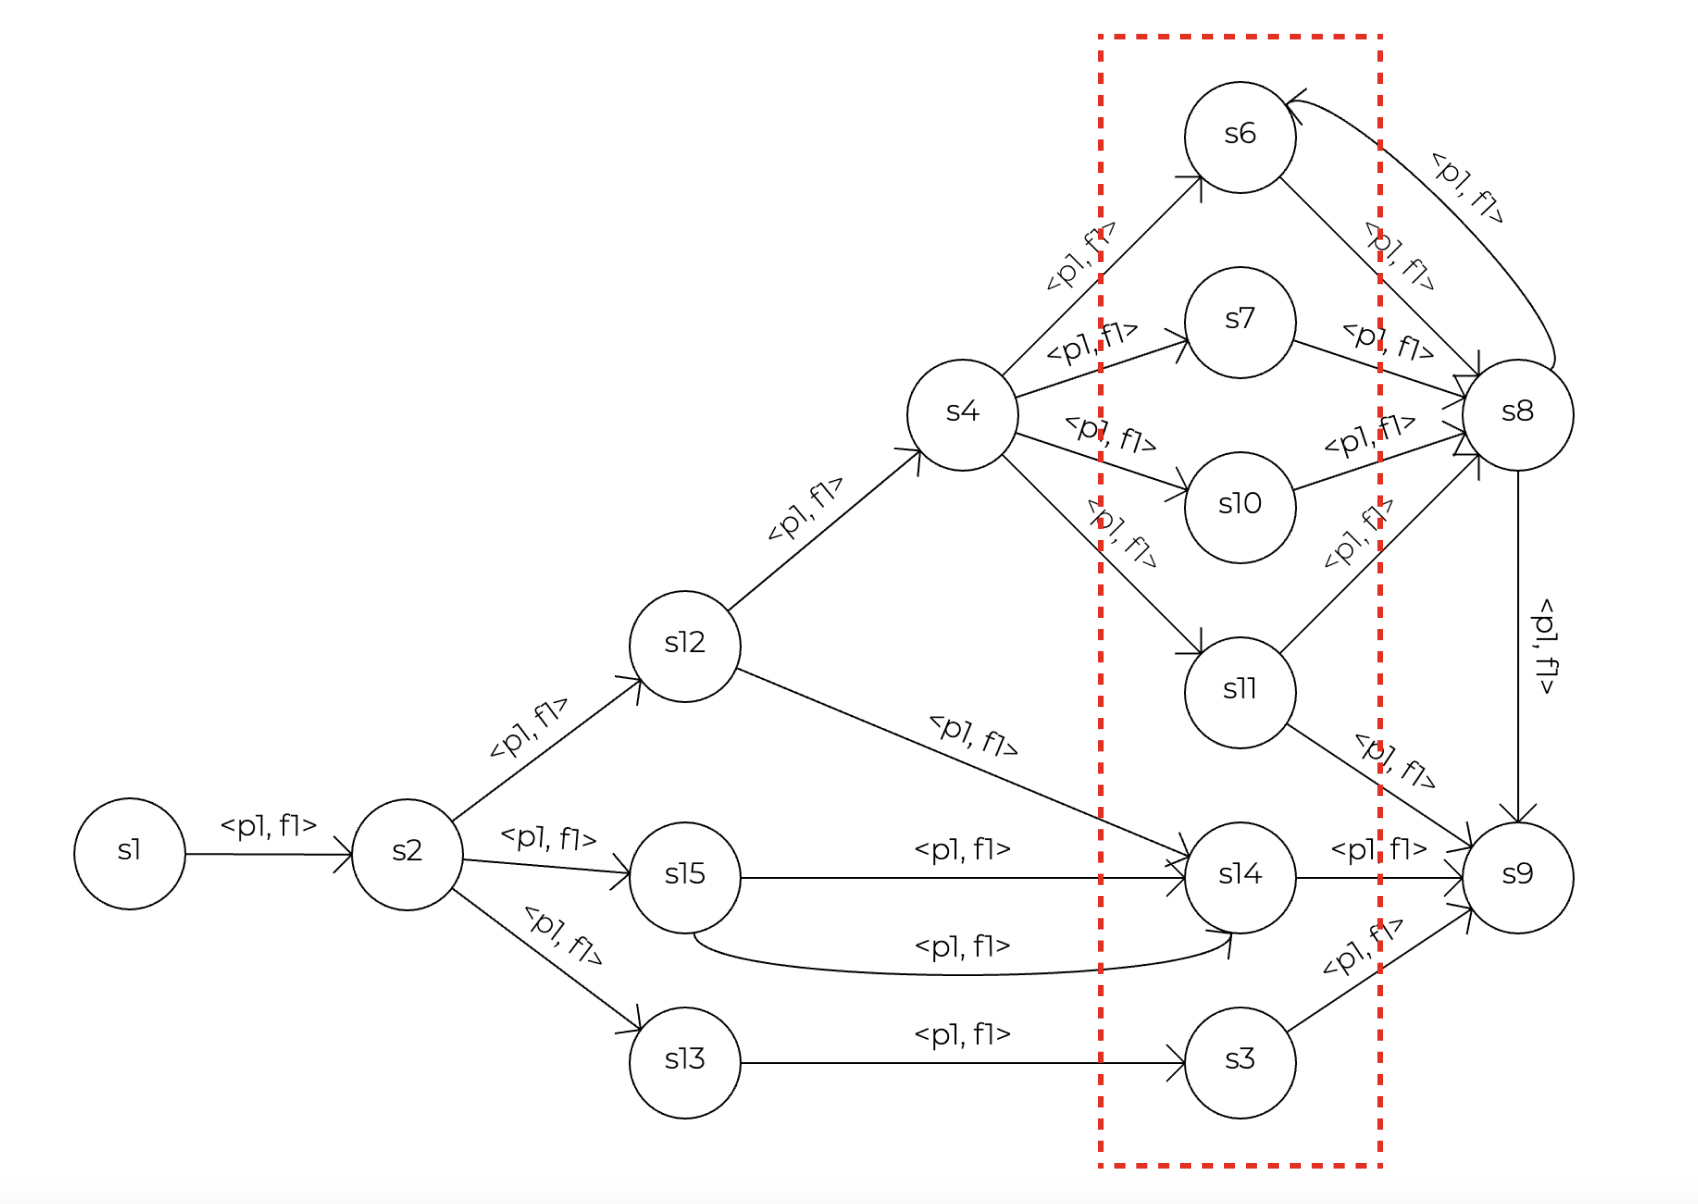
\includegraphics[width=0.85\linewidth]{ResearchNotes/rndhpc_not_edt_2021_12_04/main_graph_level5.png}}
\caption{Уровень №5 на графе}\label{fig:main_graph_level5}
\end{figure}

Обратим вниманием на то, что в объекте levels для уровня №5 содержится вершина $s_9$ которой нет на уровне №5, а она присутствует только на уровне №6. Заполнение объекта levels происходит слево-направо, то есть от меньшего
уровня к большему, например, в графе представленном выше есть связь $s_{13} \rightarrow s_3$, таким образом пока в объект levels не будет записана вершина $s_{13}$, мы не сможем записать связанную с ней вершину $s_3$.

Обратным образом происходит дублирование вершин, если обратиться к описанию графовой модели предсталвенной выше, то можно заметить такую связь: $s_1 \rightarrow s_2 \rightarrow s_{13} \rightarrow s_3 \rightarrow s_9$. При начальной инициализации объекта levels $s_1$ будет находиться на уровне 1, $s_2$ будет находиться на уровне 2 и так далее. Таким образом, вершина $s_3$ будет находиться на уровне 4, что не совсем корректно. Обработка таких ситуаций является углублением в реализацию алгоритма и в этой заметке не будет подробно описываться.

Для разрешения подобных коллизий после начальной инициализации объекта levels ``в лоб'' предусмотрено множество дополнительных проверок. Таким образом, на выходе мы получаем корректно сформированный объект levels и дополнительно формируем объект, который будет хранить информацию о вершинах которые находятся не на своем уровне, эти вершины не будут отрисовываться, но при этом они будут учитываться при выравнивании связанных с ними вершин, следовательно просто удалить такие вершины из объекта levels нельзя.

Сама визуализация вершин после формирования объекта levels также является темой отдельной заметки. На данном этапе работы над проектом сначала строится уровень содержащий наибольшее количество вершин, затем строятся оставшиеся уровни: сначала влево до уровня №1, затем вправо до самого последнего уровня.

%----------------------------------------------------------
% Атрибуты задачи
\noteattributes{}
%----------------------------------------------------------



